\chapter{Transfer Matrix Method}

\section{Introduction}

In the previous chapter, the one-dimensional scattering problem was
solved by constructing a linear system whose unknowns were the
wavefunction amplitudes inside the scattering region together with the
reflection and transmission amplitudes.

Although this approach is straightforward and robust, it is not the only
possible formulation of the problem. An alternative consists of
rewriting the discrete Schrödinger equation as a recurrence relation
connecting the wavefunction at neighboring lattice sites. This
reformulation naturally leads to the transfer matrix method.

The transfer matrix method is one of the most widely used techniques in
quantum transport. Besides its conceptual simplicity, it provides a
natural description of wave propagation through layered systems.

The main objective of this chapter is to derive the transfer matrix
directly from the tight-binding equation and to demonstrate that it
provides an alternative solution of exactly the same physical problem
studied in Chapter~1.

Although the derivation is presented for a one-dimensional chain, the
same ideas will later be generalized to matrix-valued Hamiltonians,
graphene, bilayer graphene and Bogoliubov--de Gennes systems.

%%%%%%%%%%%%%%%%%%%%%%%%%%%%%%%%%%%%%%%%%%%%%%%%%%%%%%%%%%

\section{Motivation}

The boundary-matching method solves the scattering problem by assembling
a global linear system,

\begin{equation}
	A x = b,
\end{equation}

whose dimension increases with the size of the scattering region.

The transfer matrix method follows a different philosophy. Instead of
solving for all wavefunction amplitudes simultaneously, the wavefunction
is propagated from one lattice site to the next by means of a local
linear transformation.

The entire scattering region is therefore represented by the product of
many small matrices, each describing the propagation across a single
lattice site.

This approach has several advantages.

\begin{itemize}
	\item The propagation through each site is described by the same
	      mathematical object.

	\item The total transfer matrix is obtained by successive matrix
	      multiplications.

	\item The formalism extends naturally to systems whose wavefunction
	      has internal degrees of freedom.
\end{itemize}

The last point is particularly important for the \texttt{QTransport}
project. In graphene, each longitudinal slice contains several internal
components. Nevertheless, the transfer-matrix idea remains the same.

%%%%%%%%%%%%%%%%%%%%%%%%%%%%%%%%%%%%%%%%%%%%%%%%%%%%%%%%%%

\section{From the Tight-Binding Equation to a Recurrence Relation}

The starting point is the one-dimensional tight-binding equation,

\begin{equation}
	(E-\epsilon_j)\psi_j
	+
	t\psi_{j-1}
	+
	t\psi_{j+1}
	=
	0.
	\label{eq:tm-start}
\end{equation}

The objective is to isolate the wavefunction at the next lattice site.
Rearranging Eq.~\eqref{eq:tm-start},

\begin{equation}
	t\psi_{j+1}
	=
	-
	(E-\epsilon_j)\psi_j
	-
	t\psi_{j-1}.
\end{equation}

Therefore,

\begin{equation}
	\psi_{j+1}
	=
	-
	\frac{E-\epsilon_j}{t}
	\psi_j
	-
	\psi_{j-1}.
	\label{eq:tm-recurrence}
\end{equation}

Equation~\eqref{eq:tm-recurrence} expresses the wavefunction at site
$j+1$ as a linear combination of the wavefunctions at the two preceding
sites.

%%%%%%%%%%%%%%%%%%%%%%%%%%%%%%%%%%%%%%%%%%%%%%%%%%%%%%%%%%

\section{The Local Transfer Matrix}

Introduce the two-component transfer vector

\begin{equation}
	\Phi_j
	=
	\begin{pmatrix}
		\psi_j \\
		\psi_{j-1}
	\end{pmatrix}.
	\label{eq:state-vector}
\end{equation}

Using Eq.~\eqref{eq:tm-recurrence}, one obtains

\begin{equation}
	\Phi_{j+1}
	=
	M_j
	\Phi_j,
	\label{eq:local-transfer}
\end{equation}

where

\begin{equation}
	M_j
	=
	\begin{pmatrix}
		-\dfrac{E-\epsilon_j}{t}
		 &
		-1
		\\[1ex]
		1
		 &
		0
	\end{pmatrix}.
	\label{eq:local-transfer-matrix}
\end{equation}

The original second-order difference equation has therefore been
transformed into a first-order matrix recurrence relation.

Each lattice site is represented by a single $2\times2$ matrix.

\begin{center}
	\fbox{
		\begin{minipage}{0.90\linewidth}

			\textbf{Design Decision}

			\vspace{1ex}

			The transfer matrix is introduced as a numerical representation of wave
			propagation rather than as a physical object.

			Consequently, the transfer matrix is implemented in
			\texttt{transfer.py}, while the Hamiltonian and the scattering region
			remain independent objects.

			This separation allows the same physical problem to be solved using
			different numerical techniques.

		\end{minipage}
	}
\end{center}

%%%%%%%%%%%%%%%%%%%%%%%%%%%%%%%%%%%%%%%%%%%%%%%%%%%%%%%%%%

\section{The Total Transfer Matrix}

The local transfer matrix describes the propagation across a single
lattice site. To determine the propagation through the entire scattering
region, the local matrices are multiplied successively.

For a scattering region containing $N$ sites,

\begin{align}
	\Phi_1 & = M_0\Phi_0, \\
	\Phi_2 & = M_1\Phi_1
	= M_1M_0\Phi_0,       \\
	\Phi_3 & = M_2\Phi_2
	= M_2M_1M_0\Phi_0.
\end{align}

After crossing the complete scattering region,

\begin{equation}
	\Phi_N
	=
	M
	\Phi_0,
	\label{eq:total-transfer}
\end{equation}

where

\begin{equation}
	M
	=
	M_{N-1}
	M_{N-2}
	\cdots
	M_1
	M_0.
	\label{eq:total-transfer-matrix}
\end{equation}

The matrix $M$ is the total transfer matrix of the scattering region.

\begin{center}
	\fbox{
		\begin{minipage}{0.90\linewidth}

			\textbf{Physical Insight}

			\vspace{1ex}

			The local transfer matrix describes propagation through a single lattice
			site.

			The total transfer matrix describes propagation through the entire
			device.

			This is analogous to building a complete evolution operator from many
			local evolution steps.

		\end{minipage}
	}
\end{center}

%%%%%%%%%%%%%%%%%%%%%%%%%%%%%%%%%%%%%%%%%%%%%%%%%%%%%%%%%%

\section{Boundary Conditions}

The transfer matrix propagates the wavefunction through the scattering
region. To determine the reflection and transmission amplitudes, the
lead boundary conditions must still be imposed.

For an incoming wave from the left,

\begin{equation}
	\psi_j
	=
	e^{ikj}
	+
	r e^{-ikj},
	\qquad
	j\leq -1.
	\label{eq:left-transfer}
\end{equation}

In the right lead,

\begin{equation}
	\psi_j
	=
	\tau e^{ikj},
	\qquad
	j\geq N.
	\label{eq:right-transfer}
\end{equation}

The transfer vectors at the two sides of the scattering region are

\begin{equation}
	\Phi_0
	=
	\begin{pmatrix}
		\psi_0 \\
		\psi_{-1}
	\end{pmatrix},
	\qquad
	\Phi_N
	=
	\begin{pmatrix}
		\psi_N \\
		\psi_{N-1}
	\end{pmatrix}.
\end{equation}

Using the left-lead ansatz,

\begin{equation}
	\Phi_0
	=
	\begin{pmatrix}
		1+r \\
		e^{-ik}+r e^{ik}
	\end{pmatrix}.
	\label{eq:left-vector}
\end{equation}

Using the right-lead ansatz,

\begin{equation}
	\Phi_N
	=
	\tau
	\begin{pmatrix}
		e^{ikN} \\
		e^{ik(N-1)}
	\end{pmatrix}.
	\label{eq:right-vector}
\end{equation}

Substitution into Eq.~\eqref{eq:total-transfer} gives

\begin{equation}
	\tau
	\begin{pmatrix}
		e^{ikN} \\
		e^{ik(N-1)}
	\end{pmatrix}
	=
	M
	\begin{pmatrix}
		1+r \\
		e^{-ik}+r e^{ik}
	\end{pmatrix}.
	\label{eq:transfer-boundary}
\end{equation}

This equation contains the complete scattering problem.

%%%%%%%%%%%%%%%%%%%%%%%%%%%%%%%%%%%%%%%%%%%%%%%%%%%%%%%%%%

\section{Extraction of the Reflection and Transmission Amplitudes}

Define the three boundary vectors

\begin{equation}
	\Phi_{\mathrm{in}}
	=
	\begin{pmatrix}
		1 \\
		e^{-ik}
	\end{pmatrix},
	\qquad
	\Phi_{\mathrm{ref}}
	=
	\begin{pmatrix}
		1 \\
		e^{ik}
	\end{pmatrix},
	\qquad
	\Phi_{\mathrm{out}}
	=
	\begin{pmatrix}
		e^{ikN} \\
		e^{ik(N-1)}
	\end{pmatrix}.
\end{equation}

Then the boundary equation can be written as

\begin{equation}
	M
	\left(
	\Phi_{\mathrm{in}}
	+
	r\Phi_{\mathrm{ref}}
	\right)
	=
	\tau
	\Phi_{\mathrm{out}}.
\end{equation}

Collecting the unknown amplitudes gives

\begin{equation}
	rM\Phi_{\mathrm{ref}}
	-
	\tau\Phi_{\mathrm{out}}
	=
	-
	M\Phi_{\mathrm{in}}.
	\label{eq:small-system}
\end{equation}

Equation~\eqref{eq:small-system} is a $2\times2$ linear system for the
reflection amplitude $r$ and the transmission amplitude $\tau$.

%%%%%%%%%%%%%%%%%%%%%%%%%%%%%%%%%%%%%%%%%%%%%%%%%%%%%%%%%%

\section{Implementation in QTransport}

The transfer-matrix formalism is implemented in

\begin{center}
	\texttt{src/qtransport/transfer.py}.
\end{center}

The source code follows the mathematical structure derived above:

\[
	\text{local matrix}
	\longrightarrow
	\text{total matrix}
	\longrightarrow
	\text{boundary vectors}
	\longrightarrow
	\text{scattering amplitudes}.
\]

%%%%%%%%%%%%%%%%%%%%%%%%%%%%%%%%%%%%%%%%%%%%%%%%%%%%%%%%%%

\subsection{Implementation of the Local Transfer Matrix}

The method \texttt{local\_matrix()} implements
Eq.~\eqref{eq:local-transfer-matrix}.

\inputminted[
	fontsize=\footnotesize,
	linenos,
	breaklines,
	frame=lines,
	firstline=54,
	lastline=79
]{python}{../src/qtransport/transfer.py}

The matrix element

\[
	-\frac{E-\epsilon_j}{t}
\]

appears directly in the first row of the returned NumPy array. The
second row implements the shift

\[
	(\psi_j,\psi_{j-1})
	\mapsto
	(\psi_{j+1},\psi_j).
\]

%%%%%%%%%%%%%%%%%%%%%%%%%%%%%%%%%%%%%%%%%%%%%%%%%%%%%%%%%%

\subsection{Implementation of the Total Transfer Matrix}

The method \texttt{total\_matrix()} implements the ordered product

\[
	M
	=
	M_{N-1}
	M_{N-2}
	\cdots
	M_0.
\]

\inputminted[
	fontsize=\footnotesize,
	linenos,
	breaklines,
	frame=lines,
	firstline=81,
	lastline=97
]{python}{../src/qtransport/transfer.py}

The method starts from the identity matrix, corresponding to propagation
through an empty region. Each local matrix is then multiplied from the
left, preserving the ordering required by Eq.~\eqref{eq:total-transfer-matrix}.

\begin{center}
	\fbox{
		\begin{minipage}{0.90\linewidth}

			\textbf{Computational Remark}

			\vspace{1ex}

			For a one-dimensional chain containing $N$ sites, the construction of
			the total transfer matrix requires $N$ local matrix multiplications.

			The cost therefore scales linearly with the number of sites.

		\end{minipage}
	}
\end{center}

%%%%%%%%%%%%%%%%%%%%%%%%%%%%%%%%%%%%%%%%%%%%%%%%%%%%%%%%%%

\subsection{Implementation of the Boundary Vectors}

The vectors
$\Phi_{\mathrm{in}}$, $\Phi_{\mathrm{ref}}$ and
$\Phi_{\mathrm{out}}$ are implemented by three small methods.

\inputminted[
	fontsize=\footnotesize,
	linenos,
	breaklines,
	frame=lines,
	firstline=99,
	lastline=135
]{python}{../src/qtransport/transfer.py}

Although these methods are simple, separating them from \texttt{solve()}
makes the boundary conditions explicit and improves readability.

%%%%%%%%%%%%%%%%%%%%%%%%%%%%%%%%%%%%%%%%%%%%%%%%%%%%%%%%%%

\subsection{Implementation of the Scattering Solver}

The method \texttt{solve()} constructs the final $2\times2$ system,

\[
	rM\Phi_{\mathrm{ref}}
	-
	\tau\Phi_{\mathrm{out}}
	=
	-
	M\Phi_{\mathrm{in}},
\]

and solves it using \texttt{numpy.linalg.solve()}.

\inputminted[
	fontsize=\footnotesize,
	linenos,
	breaklines,
	frame=lines,
	firstline=137,
	lastline=184
]{python}{../src/qtransport/transfer.py}

The two unknowns returned by this system are the reflection and
transmission amplitudes. They are stored in a \texttt{ScatteringResult}
object, which also provides the corresponding reflection and
transmission probabilities.

\begin{center}
	\fbox{
		\begin{minipage}{0.90\linewidth}

			\textbf{Design Decision}

			\vspace{1ex}

			The implementation separates propagation from extraction of scattering
			amplitudes.

			The total transfer matrix describes propagation through the scattering
			region, while the final $2\times2$ linear system imposes the lead
			boundary conditions.

			This separation will be useful when the scalar wavefunction is replaced
			by a vector-valued wavefunction in graphene and superconducting systems.

		\end{minipage}
	}
\end{center}


%%%%%%%%%%%%%%%%%%%%%%%%%%%%%%%%%%%%%%%%%%%%%%%%%%%%%%%%%%

%%%%%%%%%%%%%%%%%%%%%%%%%%%%%%%%%%%%%%%%%%%%%%%%%%%%%%%%%%
\section{Validation Against the Boundary-Matching Method}

Whenever a new numerical method is introduced, it is essential to verify
that its implementation correctly reproduces the expected physical
results. In the present work, the transfer-matrix method is validated by
comparing its predictions with those obtained using the
boundary-matching method developed in Chapter~1.

Although both methods originate from different mathematical
formulations, they solve exactly the same scattering problem.
Consequently, they must produce identical reflection and transmission
probabilities for every incident energy.

Denoting the reflection and transmission probabilities obtained from the
boundary-matching method by

\[
	R_{\mathrm{BM}}(E),
	\qquad
	T_{\mathrm{BM}}(E),
\]

and those obtained from the transfer-matrix method by

\[
	R_{\mathrm{TM}}(E),
	\qquad
	T_{\mathrm{TM}}(E),
\]

the following identities must hold,

\begin{align}
	R_{\mathrm{BM}}(E)
	&=
	R_{\mathrm{TM}}(E),
	\\
	T_{\mathrm{BM}}(E)
	&=
	T_{\mathrm{TM}}(E).
\end{align}

These equalities provide a much stronger validation than merely checking
probability conservation. Indeed, both implementations individually
satisfy

\[
	R(E)+T(E)=1,
\]

which confirms that each numerical method conserves probability.
However, probability conservation alone does not guarantee that the
implemented algorithm is correct.

The comparison between two completely independent numerical methods
constitutes a far more demanding validation because both algorithms
would have to contain precisely the same error in order to produce the
same incorrect result.

For this reason, the agreement between the two methods is adopted as the
primary validation criterion throughout the development of the
\texttt{QTransport} framework.

\begin{center}
	\fbox{
		\begin{minipage}{0.90\linewidth}

			\textbf{Validation Principle}

			\vspace{1ex}

			Whenever possible, every new numerical method implemented in
			\texttt{QTransport} should be compared against an independent algorithm
			that solves the same physical problem.

			Agreement between two independent implementations provides considerably
			stronger evidence of correctness than agreement with a single numerical
			calculation.

		\end{minipage}
	}
\end{center}

In the present chapter, this validation is performed by the automated
test suite. The file

\begin{center}
\texttt{tests/physics/test\_transfer\_matrix.py}
\end{center}

contains a test that compares the transmission probability computed with
the transfer-matrix solver against the result obtained with the
boundary-matching solver. The two methods agree within numerical
precision for the tested scattering region.

%%%%%%%%%%%%%%%%%%%%%%%%%%%%%%%%%%%%%%%%%%%%%%%%%%%%%%%%%%
\section{Numerical Results}

To illustrate the transfer-matrix method, we consider the transmission
of an electron through a finite one-dimensional potential barrier.

The barrier consists of twenty lattice sites whose onsite energy is
chosen as

\[
	\epsilon_j = 0.5t,
\]

while the hopping parameter is kept constant throughout the system. The
transmission probability is calculated by solving an independent
scattering problem for each incident energy in the interval

\[
	-1.9t \le E \le 1.9t.
\]

\begin{figure}[t]
	\centering
	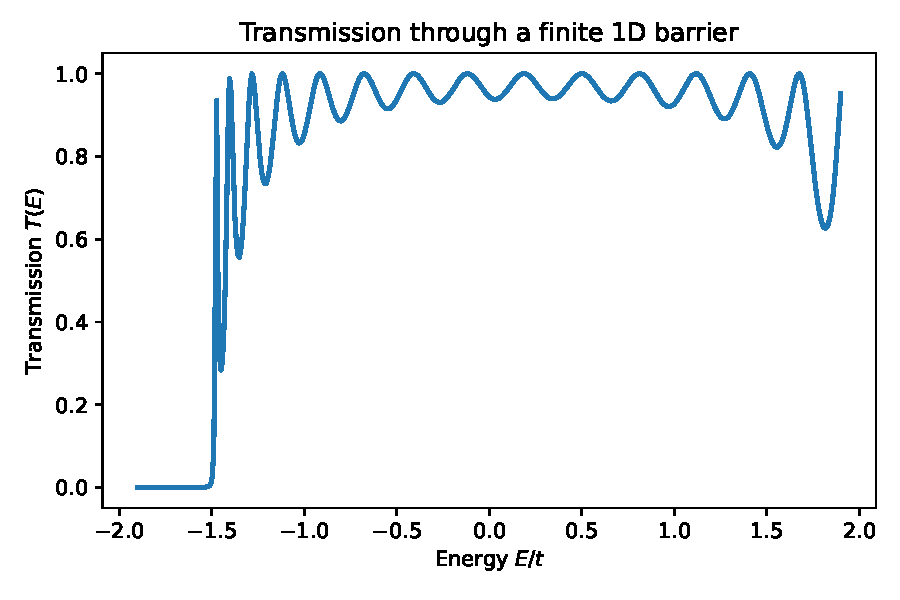
\includegraphics[width=0.82\textwidth]
	{../figures/generated/02_transfer_matrix_barrier.pdf}
	\caption{
		Validation of the transfer-matrix solver through the transmission
		probability of a finite one-dimensional barrier. The spectrum was
		computed using the transfer-matrix method and agrees, within
		numerical precision, with the boundary-matching solver introduced
		in Chapter~1.
	}
	\label{fig:tm-barrier}
\end{figure}

Figure~\ref{fig:tm-barrier} shows the transmission spectrum of the
finite barrier. Several important features can be identified.

First, the transmission coefficient satisfies

\[
	0\le T(E)\le1,
\]

as required by probability conservation.

Second, the transmission varies continuously with the incident energy.
This behavior reflects the quantum interference produced by multiple
reflections inside the finite scattering region.

Finally, the same transmission spectrum is obtained from the
boundary-matching solver. The figure therefore plays two roles: it is
the first numerical transmission result generated by the project, and it
also validates the transfer-matrix implementation against an independent
method.

\begin{center}
	\fbox{
		\begin{minipage}{0.90\linewidth}

			\textbf{Computational Experiment}

			\vspace{1ex}

			\begin{tabular}{ll}

				System &
				One-dimensional tight-binding chain \\

				Barrier length &
				20 lattice sites \\

				Barrier height &
				$\epsilon_j=0.5t$ \\

				Hopping &
				$t=1$ \\

				Energy range &
				$-1.9t\le E\le1.9t$ \\

				Numerical method &
				Transfer Matrix \\

				Example program &
				\texttt{examples/02\_transfer\_matrix\_barrier.py} \\

				Generated figure &
				\texttt{figures/generated/02\_transfer\_matrix\_barrier.pdf}

			\end{tabular}

		\end{minipage}
	}
\end{center}

%%%%%%%%%%%%%%%%%%%%%%%%%%%%%%%%%%%%%%%%%%%%%%%%%%%%%%%%%%
\section{Lessons Learned}

This chapter introduced the transfer-matrix method as a second,
independent formulation of the one-dimensional tight-binding scattering
problem.

The main mathematical lesson is that the second-order tight-binding
difference equation can be rewritten as a first-order matrix recurrence
relation,

\[
	\Phi_{j+1}
	=
	M_j
	\Phi_j.
\]

The main numerical lesson is that the full scattering region can be
represented by the ordered product of local transfer matrices,

\[
	M
	=
	M_{N-1}
	M_{N-2}
	\cdots
	M_0.
\]

The main software lesson is that propagation and boundary matching
should remain separate operations. In the implementation, the total
transfer matrix describes propagation through the scattering region,
whereas a final small linear system extracts the physical scattering
amplitudes.

The main validation lesson is that probability conservation is necessary
but not sufficient. A stronger validation is obtained by comparing two
independent algorithms that solve the same physical problem.

Finally, this chapter establishes a pattern that will be followed
throughout the rest of the project:

\[
\text{derive}
\longrightarrow
\text{implement}
\longrightarrow
\text{test}
\longrightarrow
\text{compare}
\longrightarrow
\text{plot}.
\]

\begin{center}
	\fbox{
		\begin{minipage}{0.90\linewidth}

			\textbf{Looking Ahead}

			\vspace{1ex}

			The next step is to replace the scalar wavefunction
			$\psi_j$ by a vector-valued wavefunction $\Psi_j$.
			This generalization will allow the same transfer-matrix
			architecture to describe systems with internal degrees of
			freedom, such as graphene, bilayer graphene and
			Bogoliubov--de Gennes Hamiltonians.

		\end{minipage}
	}
\end{center}

%%%%%%%%%%%%%%%%%%%%%%%%%%%%%%%%%%%%%%%%%%%%%%%%%%%%%%%%%%
\section{Reproducing the Results}

The numerical results presented in this chapter can be reproduced from
the root directory of the repository by running

\begin{minted}[
	fontsize=\footnotesize,
	breaklines,
	frame=lines
]{bash}
qtest
qpy examples/02_transfer_matrix_barrier.py
\end{minted}

The first command runs the physics tests, including the comparison
between the transfer-matrix and boundary-matching solvers. The second
command regenerates the transmission figure shown in
Fig.~\ref{fig:tm-barrier}.

The generated figure is written to

\begin{minted}[
	fontsize=\footnotesize,
	breaklines,
	frame=lines
]{text}
figures/generated/02_transfer_matrix_barrier.pdf
figures/generated/02_transfer_matrix_barrier.png
\end{minted}

This reproducibility procedure closes the loop between theory, code,
tests and numerical results.
